%--------------------
% Packages
% -------------------
\documentclass[11pt,a4paper]{article}
\usepackage[utf8x]{inputenc}
\usepackage[T1]{fontenc}
%\usepackage{gentium}
\usepackage{mathptmx} % Use Times Font
\usepackage{pdflscape}
\usepackage[numbers]{natbib}


\usepackage[pdftex]{graphicx} % Required for including pictures
\usepackage[pdftex,linkcolor=black,pdfborder={0 0 0}]{hyperref} % Format links for pdf
\usepackage{calc} % To reset the counter in the document after title page
\usepackage{enumitem} % Includes lists
\usepackage{dirtree}
\usepackage{listings}
\usepackage{jupynotex}
\usepackage{minted}

\lstset{
    basicstyle=\ttfamily,
    breaklines=true,
}


\frenchspacing % No double spacing between sentences
\linespread{1.2} % Set linespace
\usepackage[a4paper, lmargin=0.1666\paperwidth, rmargin=0.1666\paperwidth, tmargin=0.1111\paperheight, bmargin=0.1111\paperheight]{geometry} %margins
%\usepackage{parskip}

\usepackage[all]{nowidow} % Tries to remove widows
\usepackage[protrusion=true,expansion=true]{microtype} % Improves typography, load after fontpackage is selected


%-----------------------
% Set pdf information and add title, fill in the fields
%-----------------------
\hypersetup{ 	
pdfsubject = {Research Computing Coursework},
pdftitle = {Research Computing Coursework},
pdfauthor = {Laura Just Fung (lj441)}
}

%-----------------------
% Begin document
%-----------------------
\begin{document} 

\begin{center}
    \LARGE{\textbf{Research Computing Coursework Assignment}}
    \\
    \Large{{Automattic differentiation with dual numbers}}
    \\
    \large{Laura Just Fung (lj441)}
    \\
    December 18, 2024
    \\
    Word count: 1647
\end{center}


\section{Introduction}
This report discusses development of the package designed to implement automatic differentiation using dual numbers in Python. 

Dual numbers are an extension of real numbers, typically used for automatic differentiation in areas such as research computing and machine learning.

A dual number is defined like so:

\begin{equation}
    \mathrm{Dual} = a + b \epsilon
\end{equation}

Where $a$ represents the real part, and $b\epsilon$ represents the dual part. $a$ and $b$ are real numbers, and $\epsilon$ represents an infinitesimally small number such that $\epsilon^2 = 0$ but $\epsilon \neq 0$.

One application of dual numbers is their use in automatic differentiation. Any real function $f(x)$ can be extended to be a function of a dual number $f(a+b \epsilon)$ such that

\begin{equation}
    f(a + b \epsilon) = f(a) + b f'(a)\epsilon,
\end{equation}

as all terms involving $\epsilon^2$ are trivially zero. When these functions are computed over dual numbers, the dual part of the answer automatically encodes the derivative of the function. This makes them especially useful in machine learning, where derivatives are frequently calculated but can be expensive to obtain.

\section{Repository}
\subsection{Structure}
The source code for this project was organised into the following folders:

\begin{itemize}
    \item \texttt{dual\_autodiff} contains the Python implementation of the \texttt{Dual} class in \texttt{dual.py}.
    \item \texttt{dual\_autodiff\_x/src} contains the Cythonized implementation of the \texttt{Dual} class in \texttt{dual.pyc}.
    \item \texttt{tests} contains the various \texttt{.py} test modules that can be used by \texttt{pytest} \citep{pytestx.y}.
    \item \texttt{wheelhouse} contains the pure Python wheels.
    \item \texttt{dual\_autodiff\_x/wheelhouse} contains the Cythonized wheels.
\end{itemize}
\newpage
The following is a representation of the overall directory structure:

\dirtree{%
.1 dual{\_}autodiff.
.2 report.
.3 report.tex.
.3 report.pdf.
.3 \ldots.
.2 dual{\_}autodiff.
.3 {\_}{\_}init{\_}{\_}.py.
.3 dual.py.
.2 tests.
.3 test{\_}dual.py.
.3 test{\_}dual{\_}x.py.
.3 \ldots.
.2 docs.
.3 index.rst.
.3 conf.py.
.3 \ldots.
.3 {\_}build.
.4 index.html.
.4 \ldots.
.2 dual{\_}autodiff{\_}x.
.3 wheelhouse.
.4 \ldots.
.3 src.
.4 dual.pyc.
.3 {\_}{\_}init{\_}{\_}.py.
.3 setup.py.
.3 pyproject.toml.
.2 wheelhouse.
.3 \ldots.
.2 {\_}{\_}init{\_}{\_}.py.
.2 pyproject.toml.
.2 setup.py.
.2 README.md.
.2 LICENSE.
}

\subsection{Project configuration}
In order to compile this package, a \texttt{pyproject.toml} file was used. The following is its contents:
\lstinputlisting[caption={Contents of the \texttt{pyproject.toml} file.}]{../pyproject.toml}
\newpage
\section{Implementation}
In order to create a package that implements dual numbers, a class that defines what a dual number is must first be created. Afterwards, the usual binary operations (addition, subtraction, multiplication, division, exponentiation, etc.) in Python are overloaded with the dual implementations. After that, additional functions can be overloaded, including \texttt{NumPy} and \texttt{mpmath} trigonometric functions, so that dual numbers can be handled as well as real numbers. 
\subsection{Dual class}
The \texttt{Dual} class is defined and initialised like so:
\lstinputlisting[caption={Dual class initialisation in \texttt{dual.py}},language=python,linerange={5,14,22, 23}]{../dual_autodiff/dual.py}
The \texttt{real} and \texttt{dual} variables are defined as attributes of the \texttt{Dual} class that can be accessed publicly.

A dual number can be initialised as follows:
\jupynotex[2]{../dual_autodiff.ipynb}
And it produces the following output when printed:
\jupynotex[3]{../dual_autodiff.ipynb}
\newpage
\subsection{Binary operations}
Binary operations include: addition, subtraction, multiplication, division, and exponentiation. The \texttt{Dual} class allows for these operations to performed over dual numbers as well as real numbers when overloaded.
An example is as follows:
\jupynotex[4]{../dual_autodiff.ipynb}
\newpage
\subsection{Unary operations}
The unary operations implemented in the Dual class include trigonometric functions (sine, cosine, tangent), inverse trigonometric functions, hyperbolic functions, some inverse hyperbolic functions, the natural logarithm function, and the exponential function.
An sample of the functions implemented is shown below:
\jupynotex[5]{../dual_autodiff.ipynb}
\newpage
\subsection{Partial differentiation}
An additional method was added to allow for native partial differentiation with the \texttt{Dual} class. 

This was done by passing the function and its variables to the method, which acts on the variable to be partially differentiated by. All passed in variables are assumed to be dual numbers and those that are not the partially differentiating variable have their dual parts set to zero. This is so they have no effect on the derivative.

Then, the variables are passed through the given function and the derivative is returned.

An example of the method is shown below:
\jupynotex[16]{../dual_autodiff.ipynb}
\subsection{Collections}
The package was extended to allow for lists of \texttt{Dual} objects to also be operated on. Every operation and method implemented in the \texttt{Dual} class is also implemented in the \texttt{Collections} class. 

An example of this can be seen below:
\begin{landscape}
\jupynotex[17]{../dual_autodiff.ipynb}
\jupynotex[18]{../dual_autodiff.ipynb}
\jupynotex[19]{../dual_autodiff.ipynb}
\end{landscape}

\section{Local package}
The Python package is installable with \texttt{pip install -e .} from the root project folder \texttt{dual\_autodiff}. The package is importable by running in Python:

\begin{lstlisting}
    import dual_autodiff as df
\end{lstlisting}

\section{Differentiation}
Consider the function
\begin{equation}
    f(x) = \log{\sin{x}} + x^2 \cos{x}
    \label{eq:func}
\end{equation}

where $x=1.5$. The derivative can be easily calculated using \texttt{dual\_autodiff}:
\jupynotex[6]{../dual_autodiff.ipynb}

Comparing this to the analytic result

\begin{equation}
    \frac{df}{dx} = \frac{\cos{x}}{\sin{x}} + 2 x \cos{x} - x^2 \sin{x} 
\end{equation}

and various numerical methods including the central \citep{numericaldiff}

\begin{equation}
    \frac{d}{dx} f(x) \approx \frac{f(x+h) - f(x-h)}{2h},
\end{equation}

forward \citep{numericaldiff}

\begin{equation}
    \frac{d}{dx} f(x) \approx \frac{f(x+h) - f(x)}{2h},
\end{equation}

backward \citep{numericaldiff}

\begin{equation}
    \frac{d}{dx} f(x) \approx \frac{f(x) - f(x-h)}{2h},
\end{equation}

and five-point \citep{sauer_numerical_2012} equations 

\begin{equation}
    \frac{d}{dx} f(x) \approx \frac{-f(x+2h) + 8 f(x+h) - 8 f(x-h) + f(x-2h)}{12h},
\end{equation}

where accuracy mostly depends on the step size $h$. For the following comparisons in Table~\ref{tab:diffs}, a step-size of $h=1 \times 10^{-5}$ was used.

\begin{table}
    \centering
    \begin{tabular}{c|c|c}
        Method & Result (12 d.p.) & Percentage difference (\%) (12 d.p.)\\
        \hline
        \texttt{Dual} & -1.961237270553 & $0.0$\\
        Analytic & -1.961237270553 & $0.0$\\
        \hline
        Central & -1.961237270641 & $4.466\times 10^{-9}$\\
        Forward & -1.961272309059 & $1.786551078000\times 10^{-3}$\\
        Backward & -1.961202232223 & $1.786542145000 \times 10^{-3}$\\
        Five-point & -1.96123727058 & $1.353\times 10^{-9}$\\
        \hline
        Richardson central & -1.961237270561 & $4.1\times 10^{-10}$\\
        Richardson forward & -1.961248950033 & $5.955158990000\times 10^{-4}$\\
        Richardson backward & -1.961225591090 & $5.955150808000\times 10^{-4}$\\
        Richardson five-point & -1.961237270558 & $2.21\times 10^{-10}$
    \end{tabular}
    \caption{Results of each method and percentage difference of each from the \texttt{Dual} result.}
    \label{tab:diffs}
\end{table}

The Richardson extrapolation \citep{1911RSPTA.210..307R} was also used to improve the accuracy of the numerical methods. It works by taking two central approximations of the differentiation with two different step sizes $h$ and $\frac{h}{2}$ and using these to eliminate the $O(h^2)$ error term:

\begin{equation}
    D(h) = \frac{f(x+h) - f(x-h)}{2h}, 
\end{equation}

\begin{equation}
    D\biggl(\frac{h}{2}\biggr) = \frac{f(x+\frac{h}{2}) - f(x-\frac{h}{2})}{h}, 
\end{equation}

\begin{equation}
    \frac{d}{dx} f(x) \approx \frac{4 D(\frac{h}{2}) - D(h)}{3}.
\end{equation}

Comparing the numerical methods to the \texttt{Dual} result, it can be seen that with increasing step size $h$, the percentage difference gets larger, as shown in Fig.~\ref{fig:pdiff}.
\begin{landscape}
\begin{figure}
    \centering
    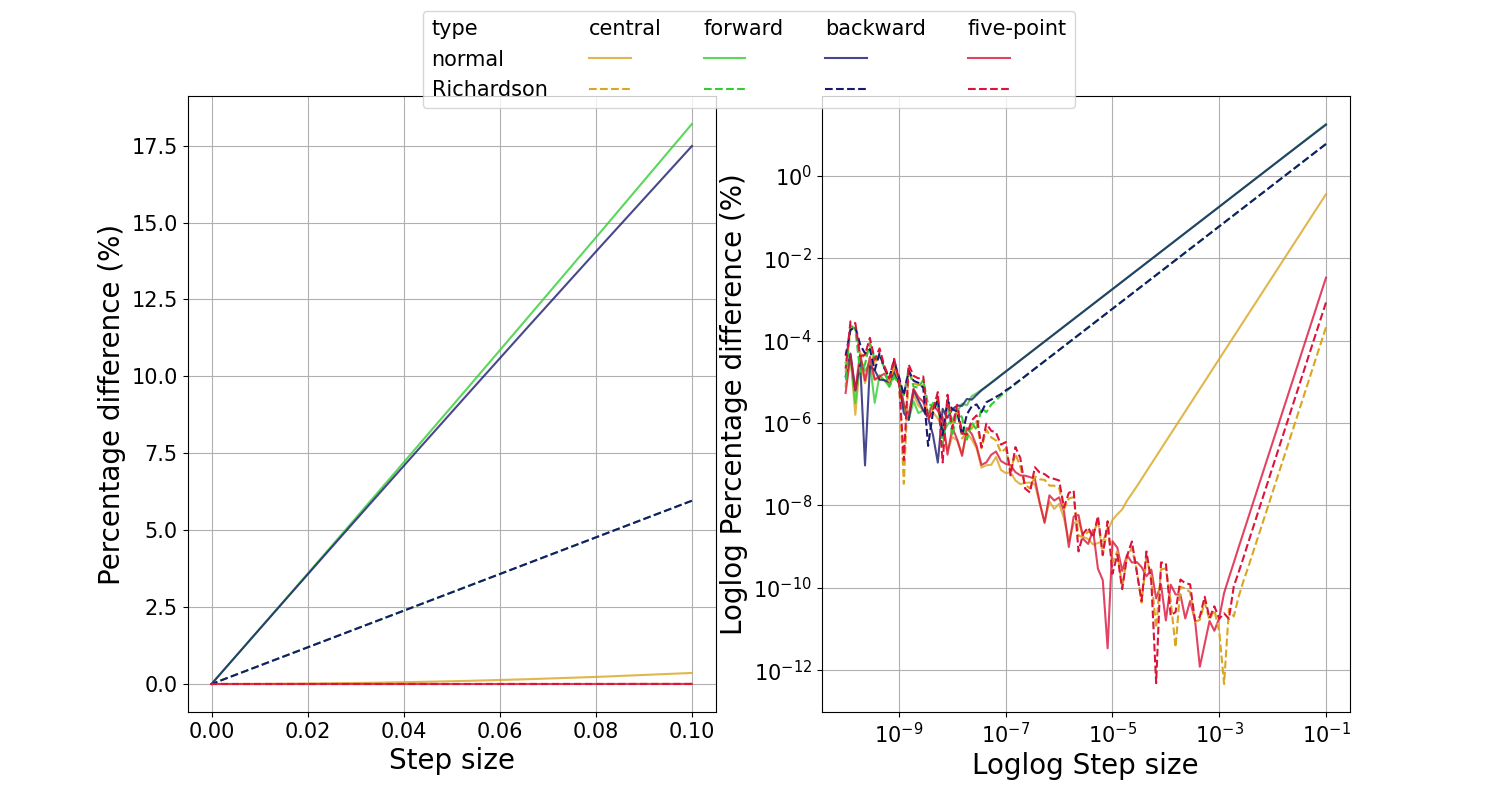
\includegraphics[width=\columnwidth, keepaspectratio]{../percentage_difference.png}
    \caption{Percentage difference between numerical and \texttt{Dual} results for the differentiation of Eq.~\ref{eq:func} at $x=1.5$ as a function of step-size $h$.}
    \label{fig:pdiff}
\end{figure}
\end{landscape}
\clearpage
\section{Test suite}
Test suites for each of the overloaded operations and functions were made in \texttt{test\_dual.py}.

Tests were made for both left and right-sided operations, ensuring that the \texttt{Dual} class can operate on and be operated on by both real and Dual numbers. Tests were also made for the unary functions to ensure that the correct differentiation of each function was made. Tests were also made for the \texttt{Collection} class, ensuring that left and right-sided operations would work on this class as well as the same unary functions implemented for the \texttt{Dual} class. Additional tests were also made for the Cythonized \texttt{Dual} and \texttt{Collection} classes.

Tests can be run using \texttt{python -m pytest tests} from within the root directory, as shown below.

\jupynotex[21]{../dual_autodiff.ipynb}

\section{Project documentation with \texttt{\textbf{Sphinx}}}
The project documentation for the \texttt{dual\_autodiff} package was done using docstrings in the \texttt{dual.py} file and compiled with \texttt{Sphinx} \citep{brandl2021sphinx}. The \texttt{index.rst} and \texttt{conf.py} files can be found in \texttt{docs} whilst the compiled \texttt{index.html} file can be found in \texttt{build}.

To use \texttt{Sphinx}, \texttt{cd} to the \texttt{docs} folder and run:

\begin{lstlisting}
    make html
\end{lstlisting}

Please note that this requires \texttt{Sphinx} which can be pip installed using the \texttt{requirements. txt} file:

\begin{lstlisting}
    pip install -r requirements.txt
\end{lstlisting}
\section{Cythonization}
Cythonization \citep{behnel2011cython} is when a Python file is compiled into optimised C/C++. This allows for fast program execution and the ability to directly call C libraries. It uses \texttt{Cython} to do this, which requires either a \texttt{.py} or \texttt{.pyx} file to Cythonize.

Within the file, it is helpful to add \texttt{cdef} before any definitions of classes or functions and to also publicly declare any variables that need to be accessed outside of the class through \texttt{cython.declare(cython.float, visibility="public")}.

Then, using a \texttt{setup.py} file, \texttt{Cython} can be called to cythonize the program. An example of this can be seen below:

\lstinputlisting[caption={The contents of the \texttt{setup.py} file.}, language=Python]{../dual_autodiff_x/setup.py}

\section{Comparison between Cythonized and pure Python programs}

The effects of Cythonization can be seen in Fig.~\ref{fig:memdiff} and Fig.~\ref{fig:timediff}. In terms of memory usage, the Cythonized \texttt{dual\_autodiff\_x} is much more efficient, while the pure Python \texttt{dual\_autodiff} takes up a lot more space.

In terms of time taken, \texttt{dual\_autodiff\_x} and \texttt{dual\_autodiff} tend to take about the same amount of time to execute operations. The main difference is that \texttt{dual\_autodiff\_x} tends to be a lot more stable, whilst \texttt{dual\_autodiff} exhibits intermittent spikes of lag.

The operations in which \texttt{dual\_autodiff\_x} shows the greatest performance boost are the basic arithmetic operations: addition, subtraction, multiplication, and division. While speedup occurs for all functions timed, as seen in Fig.~\ref{fig:speedup}, the trigonometric functions show less of an improvement, as do the exponentiation, logarithmic, and exponential functions.

\begin{figure}
    \centering
    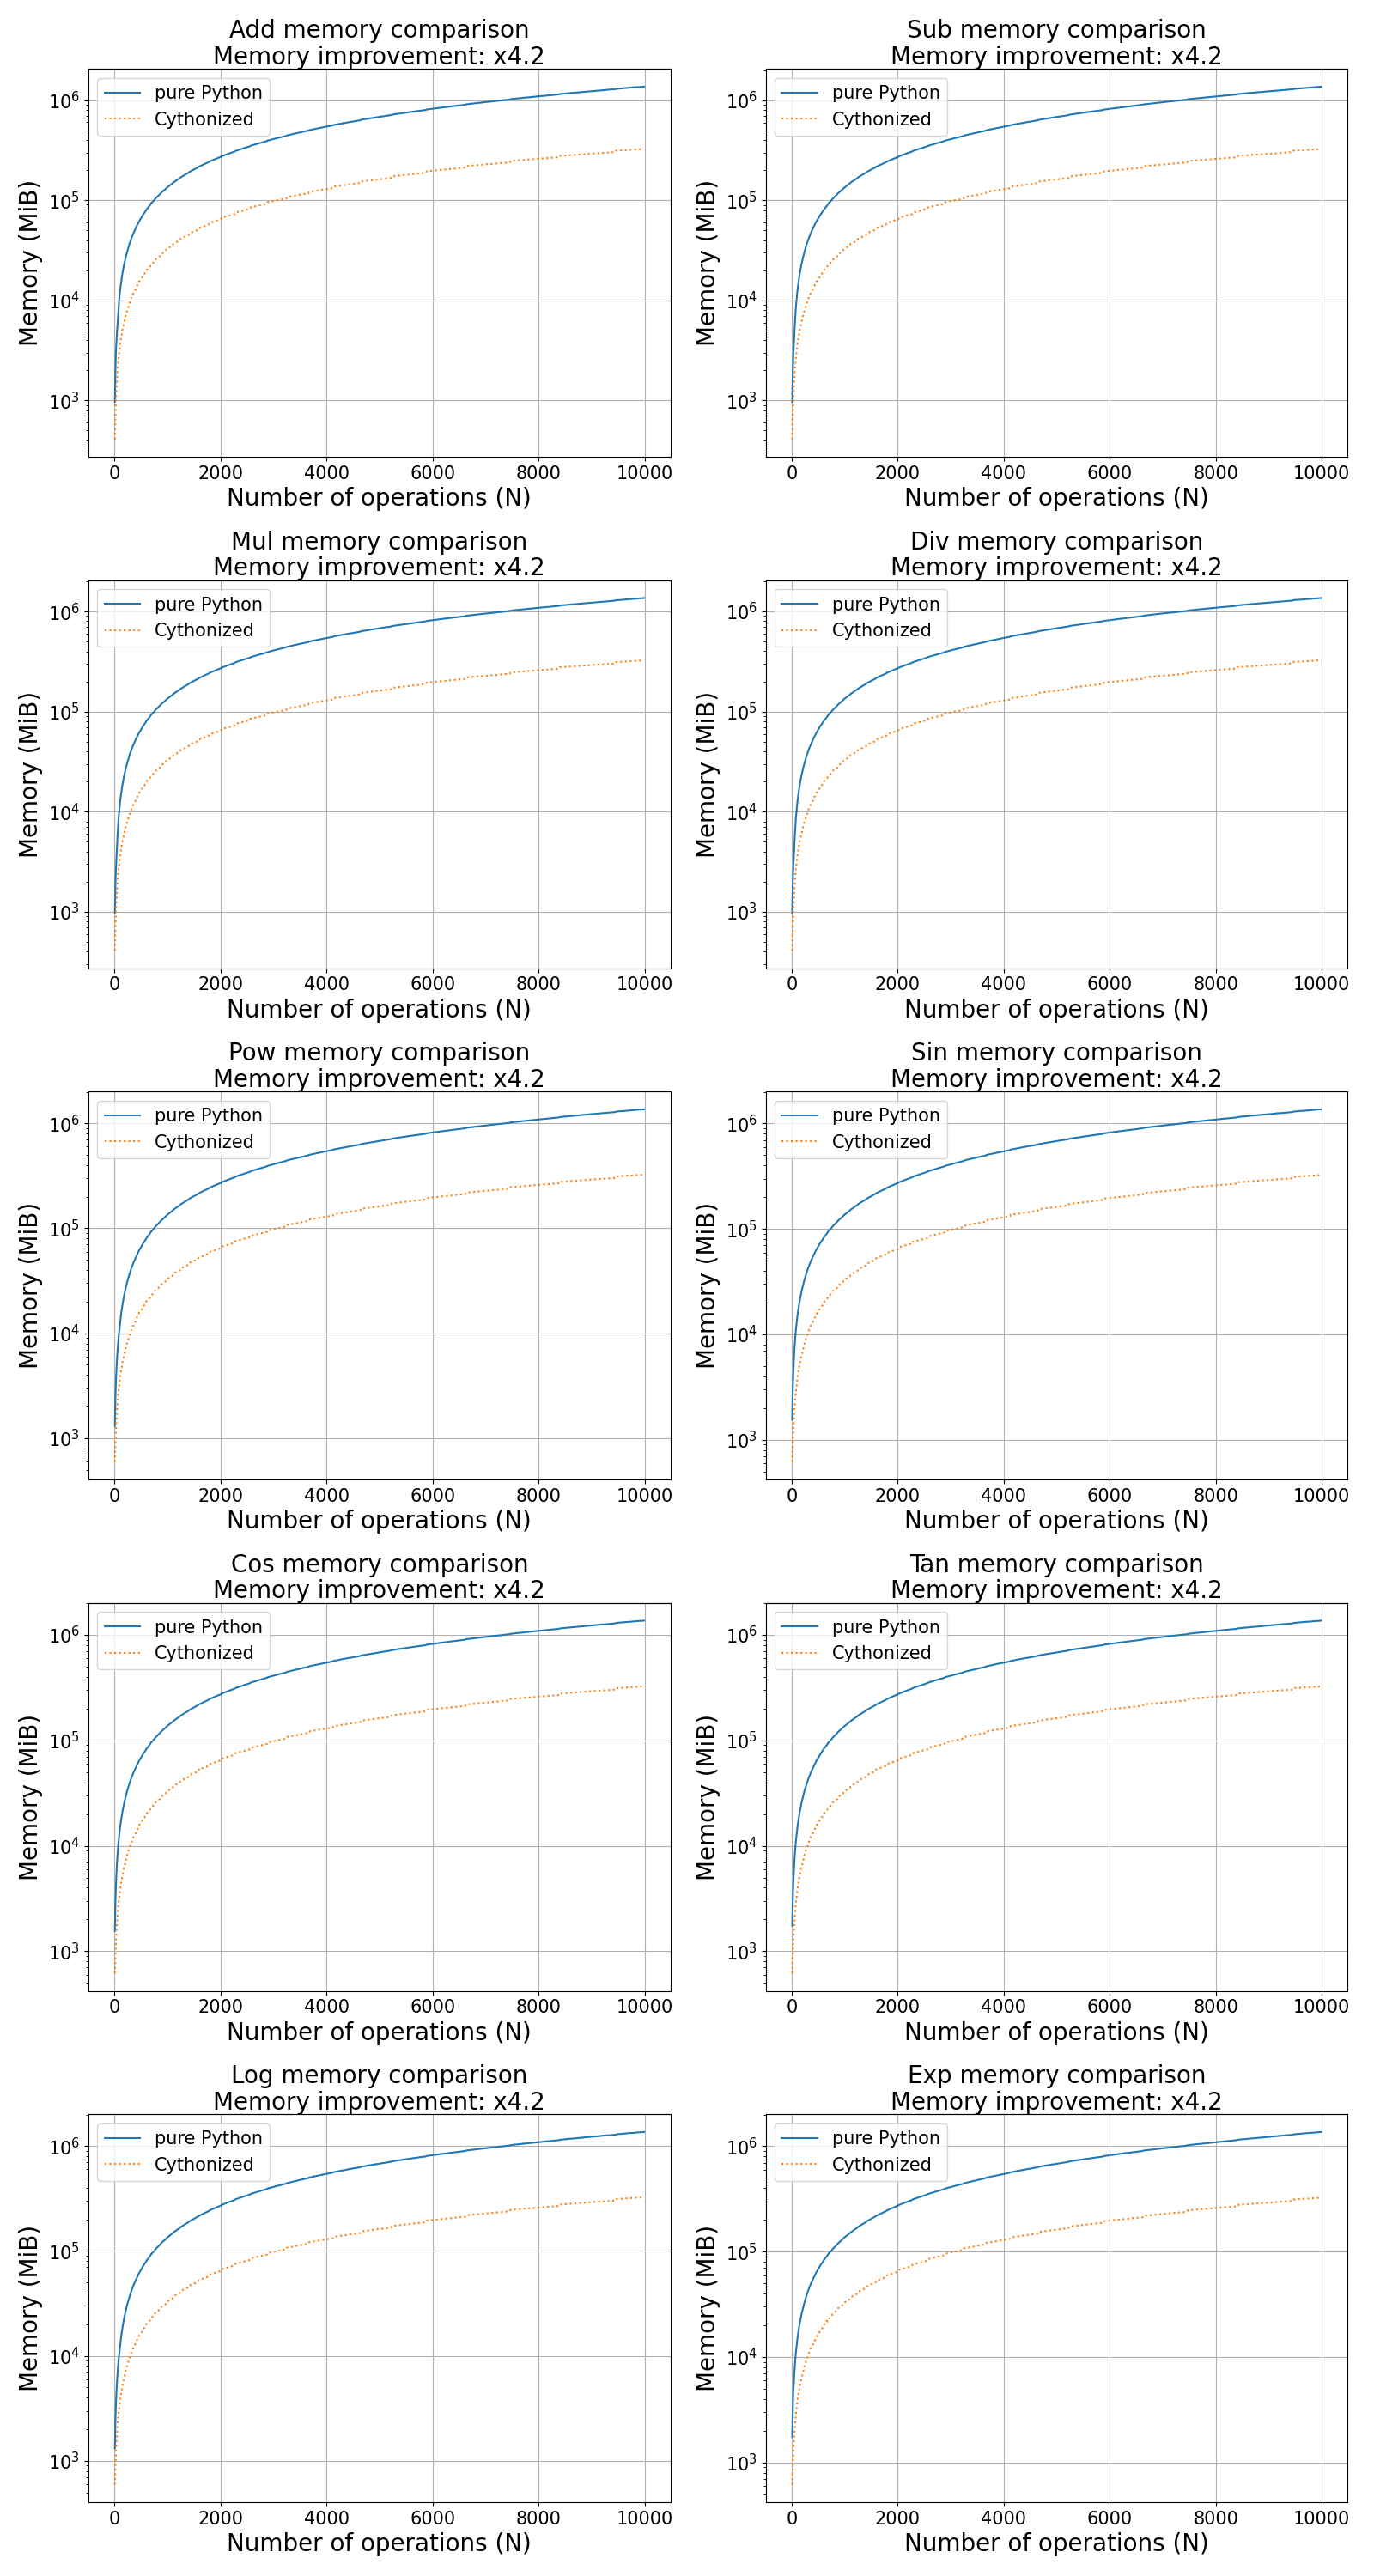
\includegraphics[width=\columnwidth, keepaspectratio]{../memory.png}
    \caption{Performance of the Cythonized and pure Python versions of the \texttt{dual\_autodiff} functions in terms of memory usage.}
    \label{fig:memdiff}
\end{figure}

\begin{figure}
    \centering
    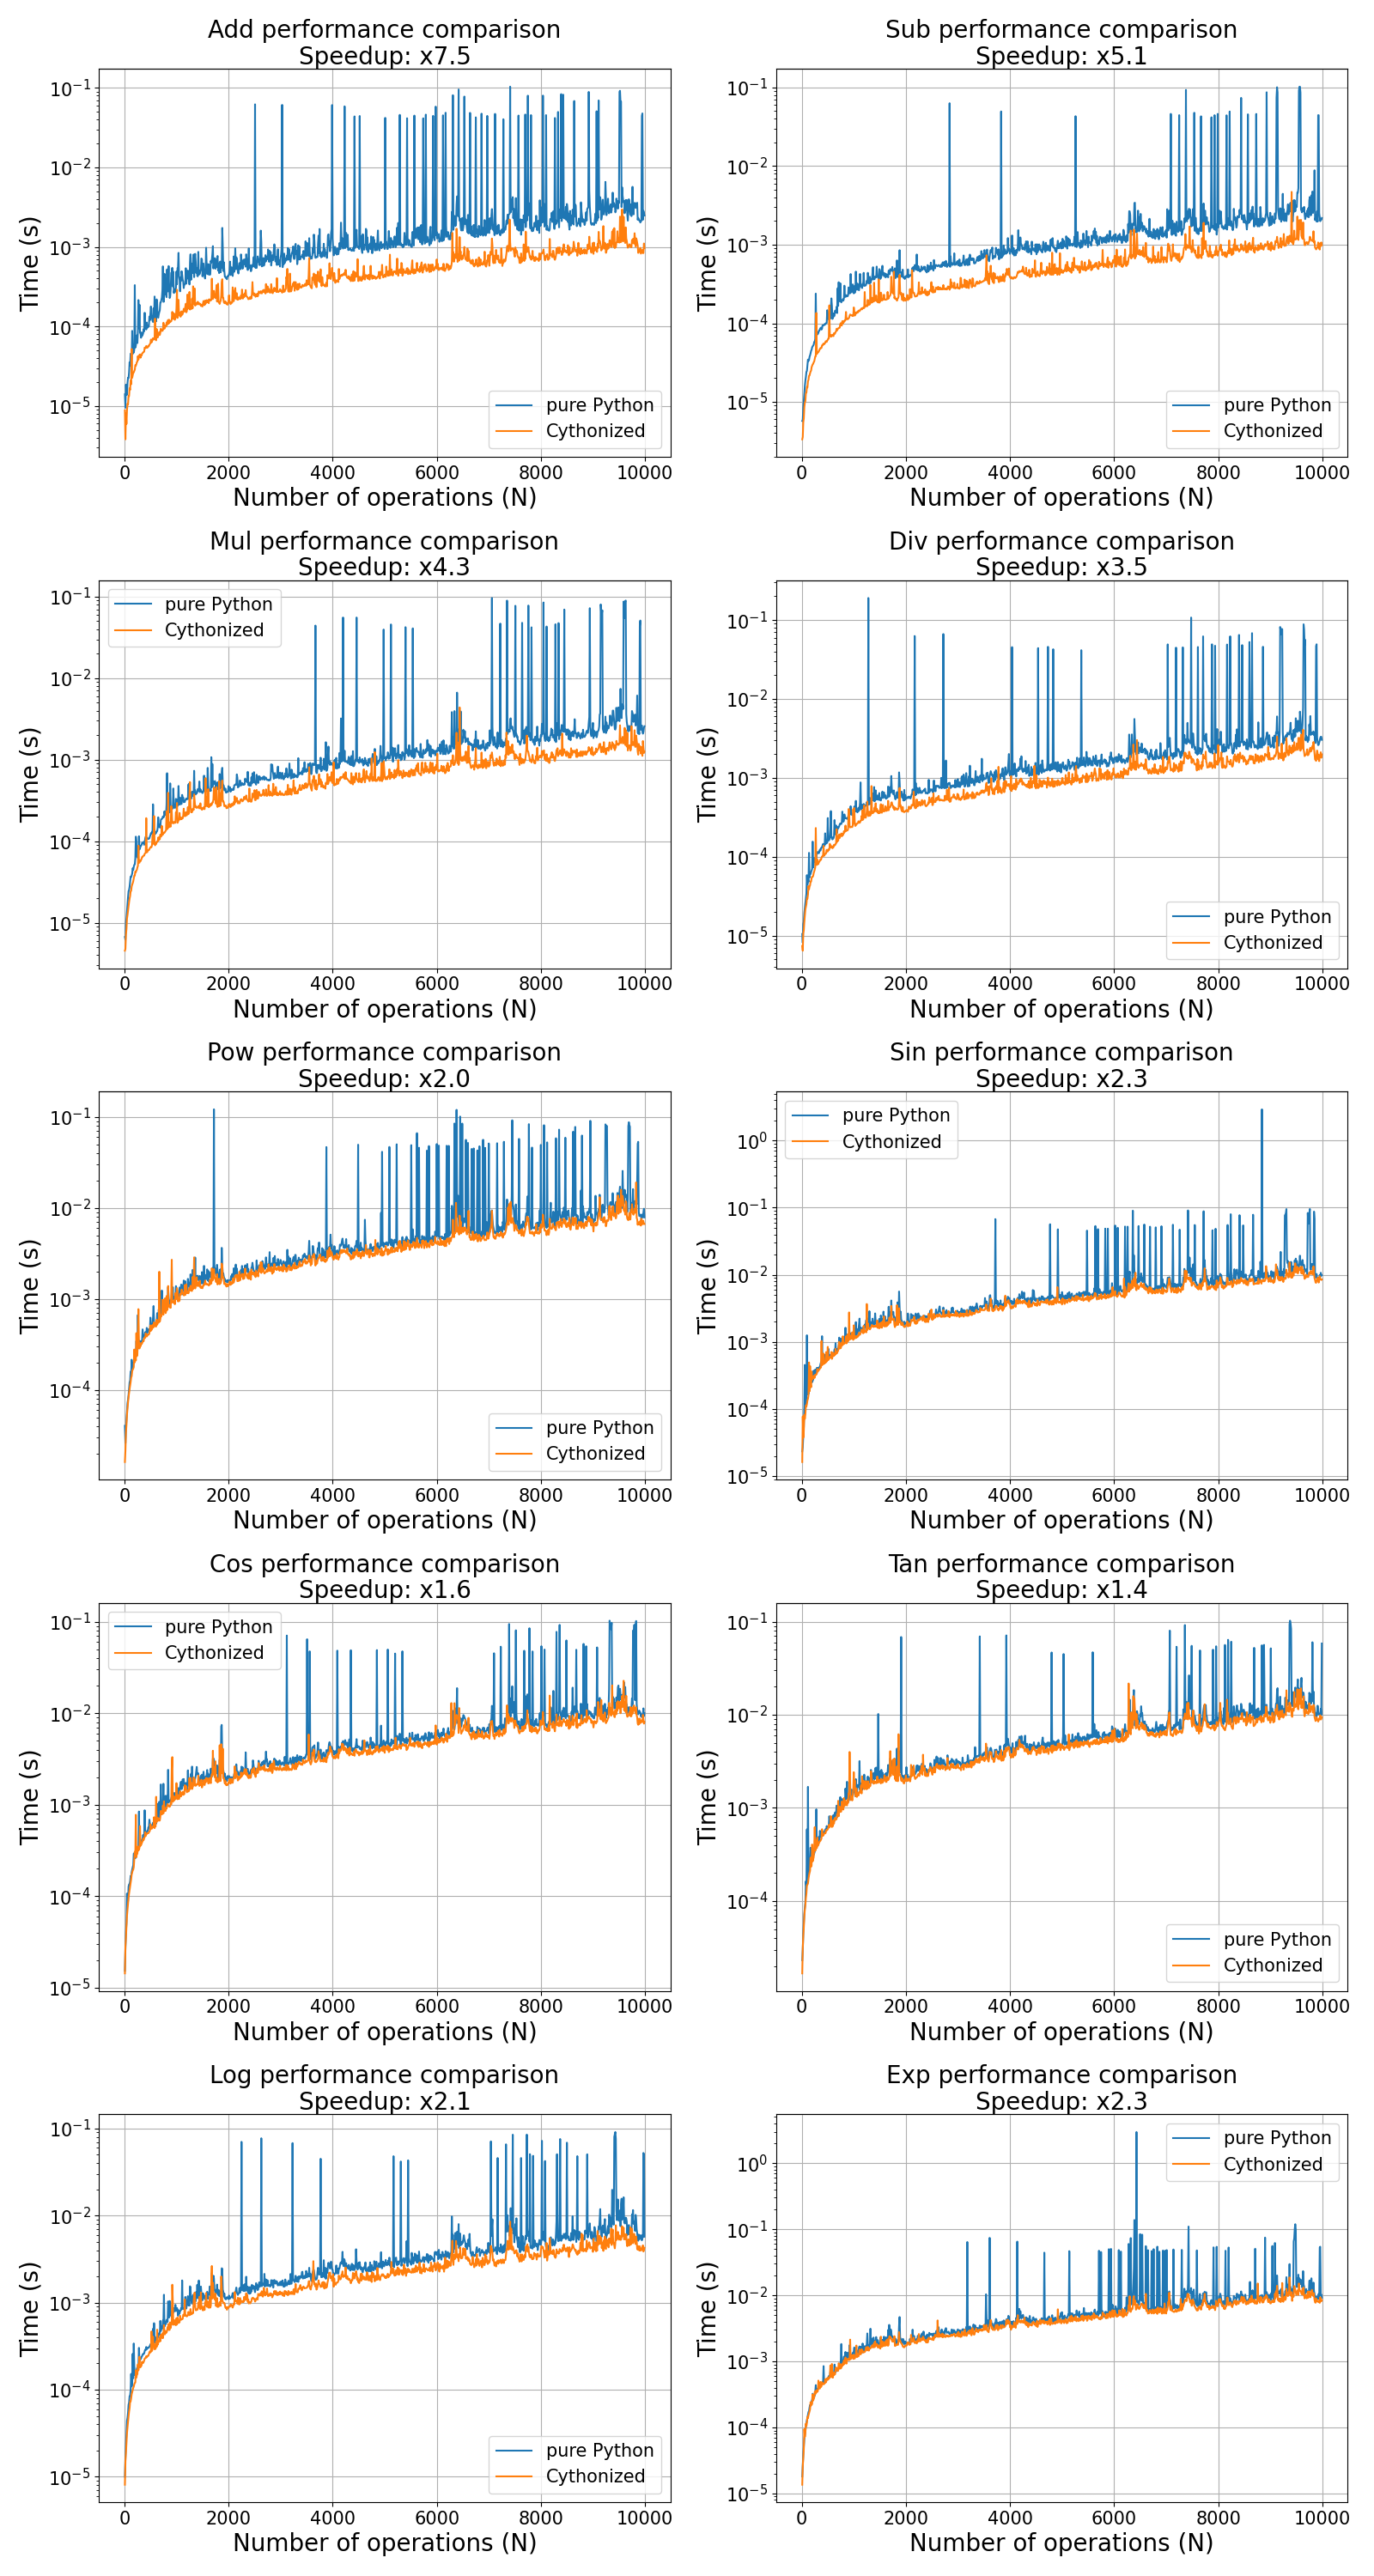
\includegraphics[width=\columnwidth, keepaspectratio]{../time.png}
    \caption{Performance of the Cythonized and pure Python versions of the \texttt{dual\_autodiff} functions in terms of time taken.}
    \label{fig:timediff}
\end{figure}

\begin{figure}
    \centering
    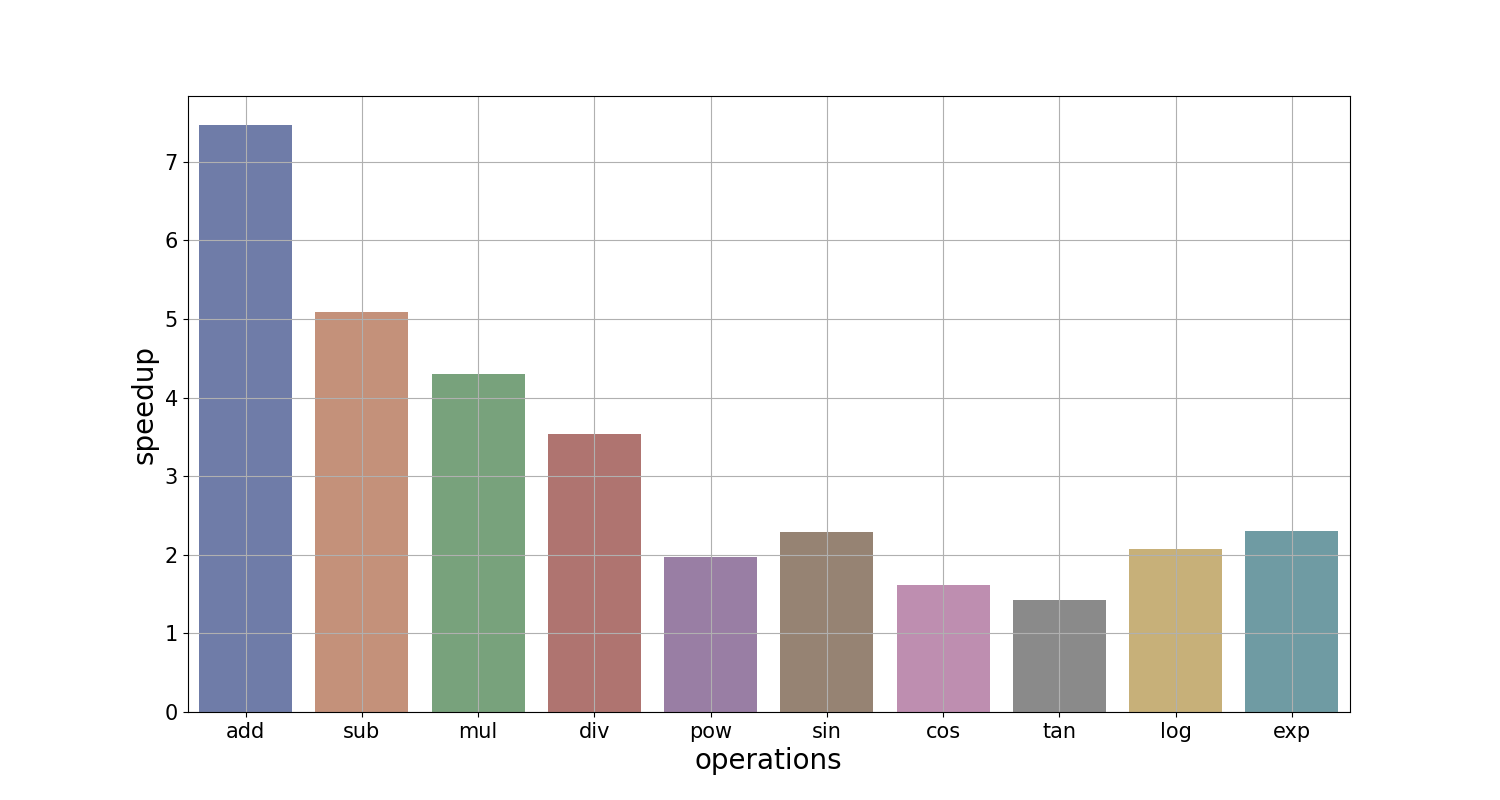
\includegraphics[width=\columnwidth, keepaspectratio]{../speedup.png}
    \caption{Averaged speedup of Cythonized version of \texttt{dual\_autodiff} compared to the time taken by the pure Python version.}
    \label{fig:speedup}
\end{figure}

\section{Wheels}

\texttt{cibuildwheel} \citep{cibuildwheel} is a package that uses Docker to create wheels specifically for different operating systems and architectures. Wheels are a way to distribute Python packages.

For the \texttt{dual\_autodiff\_x} package, two wheels were created: one for Python 3.10 in a Linux x86 64 environment, and the other for Python 3.11 in the same environment.

For this project, \texttt{tox} was used to build the wheels in the correct \texttt{Python} environment. The \texttt{MANIFEST.in} file was used to control which files were included and excluded within the wheels. Compiled Python files, \texttt{.pyc} files, were specifically excluded.

To install the wheels, download them from \texttt{dual\_autodiff\_x/wheelhouse}. Then run
\begin{lstlisting}
    pip install dual_autodiff_x/wheelhouse/dual_autodiff_x-0.0.1-cp310-cp310-manylinux_2_17_x86_64.manylinux2014_x86_64.whl
\end{lstlisting}
or
\begin{lstlisting}
    pip install dual_autodiff_x/wheelhouse/dual_autodiff_x-0.0.1-cp311-cp311-manylinux_2_17_x86_64.manylinux2014_x86_64.whl    
\end{lstlisting}
depending on whether Python 3.10 or Python 3.11 is installed.
\clearpage
\section{Docker}
A Dockerfile was created such that the tutorial notebook \texttt{dual\_autodiff.ipynb} can be run using both \texttt{dual\_autodiff} and \texttt{dual\_autodiff\_x} packages that are installed from wheels.

This can be compiled by running:
\begin{lstlisting}
    docker build -t dual_autodiff-img .
\end{lstlisting}
And then to use the Docker image:
\begin{lstlisting}
    docker run -p 8888:8888 dual_autodiff-img
\end{lstlisting}
\section{Summary}
A package that implements a dual number class for automatic differentiation was implemented in Python 3. This package was extended such that partial differentiation is natively possible, collections of \texttt{Dual} objects can be acted on by class methods, and additional trigonometric functions were added. A testing suite was added to be used by \texttt{pytest}. The package was then Cythonized to take advantage of C/C++ libraries and to allow for fast program execution. The package was also built then into wheels specifically for Python 3.10 and 3.11 in a Linux environment and uploaded to Gitlab.
\bibliographystyle{vancouver}
\bibliography{bibliography}
\appendix
\section{Use of auto-generation tools}
Auto-generation tools were used to help parse error messages throughout the project and to help format this \LaTeX\ report.

Auto-generation tools were also used for code prototyping with the \texttt{\_\_array\_ufunc\_\_} and \texttt{\_\_array\_function\_\_} methods and code alteration when Cythonizing the package.

Auto-generation tools were not used elsewhere.

\end{document}
